\documentclass{book}
\usepackage{listings}
\usepackage{hyperref}
\usepackage{verbatim}
\usepackage{amsmath}
\usepackage[backend=bibtex, sorting=none, style=numeric-comp, defernumbers]{biblatex}
\usepackage{graphicx}

\addbibresource{\jobname.bib}

\begin{document}

\section{Classification Algorithms}%

In the last chapter we took a look at the event when the targets are continuous and might take any value within a range. In this chapter we will take a look at the case when the unknown variable is a set of discreet values. This type of cases are common in the real world. A fruit may be apple, lemon or something else. We might need to go to Delhi or Bangalore. Such scenarios where the machine learning algorithm is tasked with bucketing input variables into some predefined buckets are called classification problems. In this chapter we will take a look at classification algorithms and see how we can create models in Rust.

In Rust we can create classifiers using the package \lstinline{rustlearn}. This crate contains effective implementation for a number of common machine learning algorithms. To be able to use \lstinline{rustlearn}, we will need to implement the floats as \lstinline{float32}.

\subsection{Iris Data Set}%

\paragraph{}%
For showing the usage of the classification algorithms we will be using the iris dataset\footnote{\href{https://archive.ics.uci.edu/ml/datasets/iris}{Iris Data Set}}. It is a multivariate data set with the following features.

\begin{itemize}
	\item Sepal length in cm
	\item sepal width in cm.
	\item petal length in cm.
	\item petal width in cm.
	\item classes: setosa, versicolor and virginica.
\end{itemize}

The code that is explained here is kept in the \lstinline{rustlearn_classification_tasks} folder. Inside the package create a folder \lstinline{data} and keep the csv file there.
\label{par:}

\begin{lstlisting}[language=bash,caption={iris data}]
$ head -n2 data/iris.csv
sepal_length,sepal_width,petal_length,petal_width,species
5.1,3.5,1.4,0.2,setosa
$ wc -l data/iris.csv
151 data/iris.csv # there are 150 samples in the data set.
\end{lstlisting}

Similar to before we are going to work with \lstinline{rustlearn}, \lstinline{csv}, \lstinline{rand} and \lstinline{serde}. Find these dependencies in the \lstinline{Cargo.toml} file.

\begin{lstlisting}[caption={Cargo\\.toml}]
[dependencies]
rustlearn = "0.5.0"
csv = "1.0.5"
serde = "1.0.89"
rand = "0.6"

\end{lstlisting}

\paragraph{}%
Remember that in the regression case we created a \lstinline{BostonHousing} \lstinline{struct}. In this case we are going ahead with creating a \lstinline{Flower} \lstinline{struct}.
\label{par:}

\begin{lstlisting}[caption={ml\\-utils\\/src\\/datasets\\.rs}]
extern crate serde;
#[macro_use]
extern crate serde_derive;

#[derive(Debug, Deserialize)]
struct Flower {
  sepal_length: f32, sepal_width: f32,
  petal_length: f32, petal_width: f32,
  species: String,
}
\end{lstlisting}

Here species is the label and other columns are the features. So to parse out the features and the labels we will implement \lstinline{into_feature_vector} and \lstinline{into_labels} for the \lstinline{Flower} \lstinline{struct}. Note that in case of defining the feature vector the order of the placement in the csv file is maintained. And in case of label encoding some numbers (which are arbitrary) are given to the different labels. Ideally along with a label encoding method a label decoder should also be implemented for the final response. In this case for the sake of brevity that is not shown.

\begin{lstlisting}[caption={ml\\-utils\\/src\\/datasets\\.rs}]
use std::io; use std::vec::Vec; use csv;
impl Flower {
  fn into_feature_vector(&self) -> Vec<f32> {
    vec![self.sepal_length, self.sepal_width,
    self.sepal_length, self.petal_width]
  }

  fn into_labels(&self) -> f32 {
    match self.species.as_str() {
      "setosa" => 0., "versicolor" => 1.,
      "virginica" => 2.,
      some_other => panic!("Not able to parse the label.
        Some other label got passed. {:?}", some_other),
    }
  }
}
\end{lstlisting}

We will use the amazing \lstinline{stdin} and read the package using a command similar to \lstinline{cargo run lr < data/iris.csv}. Here \lstinline{cargo run} will compile and run the binary and \lstinline{lr} is the argument after that which is enabled in the package. Take a look at \lstinline{main.rs} for all the options. So to enable that we will use the \lstinline{std::io} package and pass it to a \lstinline{rdr} variable using \lstinline{csv::Reader}. We now serialize each record to the \lstinline{Flower} \lstinline{struct} and push it to and push it to a data vector, a similar data vector that we h ave seen in the regression section. With this we will also shuffle the data for good measure.

\begin{lstlisting}[caption={chapter3\\/rustlearn\_classification\_tasks\\/src\\/logistic\_reg\\.rs}]
use ml_utils::datasets::Flower;

use csv; use rand::thread_rng;
use rand::seq::SliceRandom;
let mut rdr = csv::Reader::from_reader(io::stdin());
let mut data = Vec::new();
for result in rdr.deserialize() {
  let r: Flower = result?; // should have Box<Error> in the defn.
  data.push(r);
}
data.shuffle(&mut thread_rng());
\end{lstlisting}

Now we will be separating out the train and test datasets. The code is similar to the one in regression section except here in this case we will need to convert the vectors into \lstinline{rustlearn} sparse or dense vectors.

\begin{lstlisting}[caption={chapter3\\/rustlearn\_classification\_tasks\\/src\\/logistic\_reg\\.rs}]
use rustlearn::prelude::*;

// separate out to train and test datasets.
let test_size: f32 = 0.2;
let test_size: f32 = data.len() as f32 * test_size;
let test_size = test_size.round() as usize;
let (test_data, train_data) = data.split_at(test_size);
let train_size = train_data.len();
let test_size = test_data.len();

// differentiate the features and the labels.
let flower_x_train: Vec<f32> = train_data.iter()
  .flat_map(|r| r.into_feature_vector()).collect();
let flower_y_train: Vec<f32> = train_data.iter()
  .map(|r| r.into_labels()).collect();
let flower_x_test: Vec<f32> = test_data.iter()
  .flat_map(|r| r.into_feature_vector()).collect();
let flower_y_test: Vec<f32> = test_data.iter()
  .map(|r| r.into_labels()).collect();

// Convert the vectors to a dense matrix or a sparse matrix
let mut flower_x_train = Array::from(flower_x_train);
flower_x_train.reshape(train_size, 4);
let flower_y_train = Array::from(flower_y_train);
let mut flower_x_test = Array::from(flower_x_test);
flower_x_test.reshape(test_size, 4);
\end{lstlisting}

We should now be able to train the data on \lstinline{rustlearn} models.
\label{sub:iris_data_set}

\subsection{Logistic Regression}%
\paragraph{}%
Logistic Regression is a popular classification technique in which a logit function is used to model a binary dependent variable. The assumption for the dependent variable is that it follows Bernoulli distribution. While OLS regression is a distance-minimizing approximation method, estimation of parameters is done using the maximum likelihood method. Maximizing the likelihood function determines the parameters that are most likely to produce the observed data.
\label{par:}
\paragraph{}%
Below is the equation of the logit function. This function can take any real valued integer and map it to values between 0 and 1. If the curve goes to positive infinity, the output is assumed to be a success and failure for the opposite case. As an input case the input that is given as the logarithm of the odds $p/(1-p)$ where p is the probability.

\begin{equation}
	\frac{1}{1 + \exp^t}
\end{equation}

If t is assumed to be a function of the form $t = \beta_0 + \beta_1 x_1 + \dots$. This can now be replaced in the above equation as

\begin{equation}
	\frac{1}{1 + \exp^{\beta_0 + \beta_1 x_1 + \dots}}
\end{equation}
\label{par:}

\paragraph{}%
Taking this function the regression coefficients are estimated using maximum likelihood estimation.
\begin{equation}
	\hat{\beta} = \min_{\beta} - LL(\beta; y, X)
\end{equation}

Unlike regression, for normally distributed residuals, it is not possible to find a closed form solution that maximize the function. So an iterative approach has to be used. One of the popular iterative approaches is Gradient Descent which has been discussed in the regression section. So gradient descent follows the recursion
\begin{equation}
	\beta_{t + 1} = \beta_t - \eta_t \Lambda F(\chi_t)
\end{equation}

\label{par:}

\paragraph{}%
One of the ts of Gradient Descent is Stochastic Gradient Descent. The gradient of the loss is estimated each sample at a time and the model is updated along the way with a decreasing learning rate. So essentially instead of updating the weights only at the end of each iteration the weights are updated at each sample stage for each non zero features. So essentially SGD can be taken as a moving average of some sequence that changes with data.

Something similar to below.
\begin{equation}
	\beta_{t + 1} = \beta_t - \eta_t \Lambda f_{i_t}(\chi_t)
\end{equation}
$f_i$ being the individual sample function maintained independently. This may be done using a hash function of the weights.
\label{par:}

\paragraph{}%
Adagrad or adaptive gradient allows the learning rate to adapt based on parameters. It performs larger updates for sparse parameters and smaller updates for dense parameters. Thus it is well suited for sparse data. Another advantage is that it eliminates the need to tune the learning data. Each parameter has its own learning rate and due to the peculiarities of the algorithm the learning rate is monotonically decreasing\cite{WEBSITE:2}.
\label{par:}
\paragraph{}%
Apart from the previous methods to improve the performance of the training algorithm, we also need to take care of how we can make the resulting model have better prediction performance on out of sample data. One of the techniques to achieve this is through regularization. L1 or Lasso Regression adds absolute value of coefficient as penalty term to the loss function. While in L2 or Ridge Regression, the squared magnitude of coefficients is added to the loss function. This should reduce the overfitting of the algorithm on the training data. The idea is that if a feature does not occur enough number of times in the training dataset, it will be assigned very high coefficient by the Logistic regression. The predictive power of the feature may not be that high in the unseen data. To add regularization we will need to add a term
\begin{equation}
	\hat{\beta} = \min_{\beta} - LL(\beta; y, X) + \lambda R(\beta)
\end{equation}
This R term can be either the Manhattan distance in which case it is L1 regularization or the Euclidean distance in which case it is the L2 regularization\cite{WEBSITE:3}.
\begin{align}
	R(\beta) & = || \beta_1 || = \sum_{i=0}^{n}|\beta_i| \\
	R(\beta) &= \frac{1}{2}|| \beta_1 ||_2^2 = \frac{1}{2}\sum_{i=0}^{n}|\beta_i^2| \\
\end{align}
\label{par:}

\paragraph{Model Training}%
To implement model training in \lstinline{rustlearn} we call the \lstinline{Hyperparameter} module from \lstinline{linear_models} and can pass various parameters such as learning rate, l1 and l2 penalties and if it is a multilabel classification or binary classification.

\begin{lstlisting}[caption={chapter3\\/rustlearn\_classification\_tasks\\/src\\/logistic\_reg\\.rs}]
use rustlearn::linear_models::sgdclassifier::Hyperparameters as lr;
let mut model = lr::new(4)
  .learning_rate(0.1).l2_penalty(0.5)
  .l1_penalty(0.0).one_vs_rest();
let num_epochs = 100;
for _ in 0..num_epochs {
  model.fit(&flower_x_train, &flower_y_train).unwrap();
}
\end{lstlisting}
Running the for loop on the model is equivalent to training the model for multiple epochs.
\label{par:model_training}

\label{sub:logistic_regression}

\subsection{Decision Trees}%
Let us try to redefine the classification problem and understand it from a different perspective. In a classification problem, we have a training sample of $n$ observations on a class variable $Y$ that takes values $1, 2, ..., k$ and $p$ predictor variables, $X_1, X_2, ..., X_p$ Our goal is to find a model for predicting the values of Y for new X values. We can think of this problem as simply a partition of the X-space into $k$ disjoint sets, $A_1, A_2, ..., A_k$, such that the predicted value of Y is j if $X$ belongs to $A_j$, for $j = 1, 2, ..., k$. Classification trees take this approach. They yield rectangular sets $A_j$ by recursively partitioning the data set one $X$ variable at a time. This makes the sets easier to interpret. A key advantage of the tree structure is its applicability to any number of variables. 

The key idea is:

\begin{enumerate}
	\item Grow an overly large tree by using forward selection. At each step, find the best split. Grow until all terminal nodes either
		\begin{enumerate}
			\item have $< n$ data points,
			\item all nodes in a node have the same outcome. If this happens the node is said to be "pure".
		\end{enumerate}
	\item Prune the tree back, creating a nested sequence of trees, decreasing in complexity.
\end{enumerate}

A problem in tree construction is how to create the training data to determine the binary splits of $\chi$ into smaller and smaller pieces. The fundamental idea is to select each split in the subset so that the data in each of the descendant subsets are "purer" than the data in the parent subset. For this idea to work we will need some definition of "impurity" during training.

One measure of impurity can be the Gini coefficient. If the target is a classification outcome taking on values $0, 1, ..., k-1$ for node m, representing a region $R_m$ with $N_m$ observations, let

\begin{equation}
	p_{mk} = \frac{1}{N_m} \sum_{x_i \in R_m} I(y_i = k)
\end{equation}

be the proportion of class $k$ observations in node $m$ then the Gini coefficient is measured as

\begin{equation}
	H(\chi_m) = \sum_{k} p_{mk}(1-p_{mk})
\end{equation}

where $\chi_m$ is the training data in the node $m$.

Implementing decision trees in \lstinline{rustlearn} can be done with the below code. It supports CART algorithm for both dense and sparse data and features are selected using reduction in Gini impurity\cite{WEBSITE:4} .

\begin{lstlisting}[caption={chapter3\\/rustlearn\_classification\_tasks\\/src\\/trees\\.rs}]
use rustlearn::trees::decision_tree;
let mut tree_params = decision_tree::Hyperparameters::new(
  flower_x_train.cols());
tree_params.min_samples_split(10)
 .max_features(4).min_samples_split(5)
 .max_depth(40).one_vs_rest();
\end{lstlisting}

\label{sub:Decision trees}

\subsection{Random Forest}% TODO: write theory for bagging.
As an improvement of decision trees is the Random Forest. In this case an ensemble of trees is grown and voting is done among them to get the most popular class. The trees are a combination of tree predictors such that each tree depends on the values of a random vector sampled independently and with the same distribution for all trees in the forest. The generalization for the forests converges to a limit as the number of trees in the forest becomes large\cite{WEBSITE:7} .

To implement random forests in \lstinline{rustlearn} we will need to pass the previous decision trees variable with the parameters to the random forest \lstinline{hyperparameter} module so that a collection of trees can be built.

\begin{lstlisting}[caption={chapter3\\/rustlearn\_classification\_tasks\\/src\\/trees\\.rs}]
use rustlearn::ensemble::random_forest::Hyperparameters as rf;
let mut model = rf::new(tree_params, 10)
  .one_vs_rest();
model.fit(&flower_x_train,
          &flower_y_train)
  .unwrap();
\end{lstlisting}
\label{sub:random_forest}

\subsection{XGBoost}%
To get even better at creating a good classification model using trees, one idea is to assemble a series of weak learners to convert them into a strong classifier. XGBoost means Extreme Gradient Boosting, so lets take those terms apart one by one. In boosting the trees are built sequentially so that each subsequent tree aims to reduce the errors of the previous tree. Each tree learns from its predecessors and updates the residual errors. Hence the tree that learns next in the sequence will learn from an updated version of the residuals. So the $t$ iteration tries to fit a tree $f_t$ over all $n$ examples which minimize the following objective.

\begin{equation}
	\sum_{i=1}^{n} [g_i f_t(x_i) + \frac{1}{2}h_i f_t^2(x_i)]
\end{equation}
where $g_i$, $h_i$ are first order and second order derivatives over our previous best estimation $\hat{y}$ from iteration $t-1$.

The tree ensemble model includes functions as parameters and cannot be optimized using traditional optimization methods in Euclidean space. Hence gradient descent is used to minimize the loss function. This can be done over all possible splits in a tree. This is called the Exact Greedy algorithm and is used in many Gradient Boosting Tree algorithms. However it is impossible to enumerate over all possible splits when the data does not fit into memory. To support effective gradient tree boosting an approximate algorithm is used. So taking the previous equation when building $f_t$ and considering a specific feature $k$ in a specific split, only some split candidates are evaluated. The goal is to find candidate split points $s_{k1}, s_{k2}, ..., s_{kl}$, such that

\begin{equation}
	|r_k(s_{k, j}) - r_k(s_{k, j+1})| < \epsilon, s_{k1} = \min_i \chi_{ik}, s_{kl} = \max_i \chi_{ik}
\end{equation}

where $r$ is the ranking function (essentially we are sorting all the examples) and $\epsilon$ is the approximation factor. The second derivative is then added and the split candidate is only considered if the sum changes more than $\epsilon$. This results in a weighted quantization\cite{WEBSITE:10}.

It must be remembered that the base learner in boosting are weak learners in which the bias is high, and the predictive power is just tad better than random guessing. Each of these weak learners contribute some vital information towards labelling, thus enabling the boosting technique to produce a strong learner by effectively combining these weak learners. The final strong learner brings down both the bias and the variance.

In contrast to Random Forest, where the trees are grown to the maximum extent, boosting makes use of trees with fewer splits. Such small trees, which are not very deep, are highly interpretable. Cross-validation is an important step in boosting as this is used to find optimal parameters such as number of tress or iterations, the rate at which the gradient boosting learns, and the depth of the tree. 

\paragraph{Parameters}%
Before running XGBoost, we must set three types of parameters: general parameters, booster parameters and task parameters\cite{Chen:2016:XST:2939672.2939785} .

\begin{itemize}
	\item {\bf General parameters} relate to which type of booster we are using to do boosting, commonly they are tree models or linear models.
	\item {\bf Booster parameters} depend on which booster we have chosen
	\item {\bf Learning task parameters} decide on the learning scenario. For example, regression tasks may use different parameters with ranking tasks.
\end{itemize}
\label{par:parameters}

\paragraph{Rust-XGBoost}%
In this case instead of \lstinline{rustlearn} we will be using the \lstinline{rust-xgboost} library \footnote{\href{https://github.com/davechallis/rust-xgboost}{Rust XGBoost Source}}. The full code is kept in the package \lstinline{iris_classification_xgboost} for reference. This library is a wrapper around the XGBoost library \footnote{\href{https://github.com/dmlc/xgboost/}{Original C++ based XGBoost source}}.

In this case we will need to have \lstinline{xgboost = "0.1.4"} which is a wrapper over \lstinline{XGBoost-v0.82}. In the \lstinline{main.rs} we will call the relevant modules.

\begin{lstlisting}[caption={chapter3\\/iris\_classification\_xgboost\\/src\\/main\\.rs}]
use xgboost;
use xgboost::{parameters, DMatrix, Booster};
\end{lstlisting}

The other data preprocessing steps are the same as we have used in the previous sections for logistic regression for the Iris data set. Once the vectors \lstinline{flower_x_train}, \lstinline{flower_y_train}, \lstinline{flower_x_test}, and \lstinline{flower_y_test} vectors are created we will need to convert it to XGBoost compatible vectors though. The \lstinline{x} vectors are converted to \lstinline{DMatrix} and the corresponding labels are set.

\begin{lstlisting}[caption={chapter3\\/iris\_classification\_xgboost\\/src\\/main\\.rs}]
let mut dtrain = DMatrix::from_dense(&flower_x_train, train_size).unwrap();
dtrain.set_labels(&flower_y_train).unwrap();

let mut dtest = DMatrix::from_dense(&flower_x_test, test_size).unwrap();
dtest.set_labels(&flower_y_test).unwrap();
\end{lstlisting}

Now we will set the XGBoost parameters. First the objective function will be set to Multilabel Softmax as the number of labels are more than 2.  Then we will set the tree based learning model's parameter. These are utilised in setting the booster configuration.

\begin{lstlisting}[caption={chapter3\\/iris\_classification\_xgboost\\/src\\/main\\.rs}]
let lps = parameters::learning::LearningTaskParametersBuilder::default()
  .objective(parameters::learning::Objective::MultiSoftmax(3))
  .build().unwrap();
let tps = parameters::tree::TreeBoosterParametersBuilder::default()
  .max_depth(2).eta(1.0)
  .build().unwrap();
let bst_parms = parameters::BoosterParametersBuilder::default()
  .booster_type(parameters::BoosterType::Tree(tps))
  .learning_params(learning_params)
  .verbose(true).build().unwrap();
\end{lstlisting}

After that we will specify which matrices are for training and which for testing. This will be passed to a configuration object that will be utilised during the training.

\begin{lstlisting}[caption={chapter3\\/iris\_classification\_xgboost\\/src\\/main\\.rs}]
let ev = &[(&dtrain, "train"), (&dtest, "test")];
let params = parameters::TrainingParametersBuilder::default()
  .dtrain(&dtrain).boost_rounds(2)
  .booster_params(bst_parms)
  .evaluation_sets(Some(ev))
  .build().unwrap();
let booster = Booster::train(&params).unwrap();
\end{lstlisting}

Now the predictions can be taken and compared with the actual values.

\begin{lstlisting}[caption={chapter3\\/iris\_classification\_xgboost\\/src\\/main\\.rs}]
let preds = booster.predict(&dtest).unwrap();
let labels = dtest.get_labels().unwrap();

// find the accuracy
let mut hits = 0;
let mut correct_hits = 0;
for (predicted, actual) in preds.iter().zip(labels.iter()) {
  if predicted == actual {
    correct_hits += 1;
  }
  hits += 1;
}
assert_eq!(hits, preds.len());
println!("accuracy={} ({}/{} correct)",
  correct_hits as f32 / hits as f32, correct_hits, preds.len());
\end{lstlisting}

The accuracy should be around 93-96\%.

\label{par:rust_xgboost}

\label{sub:xgboost}

\subsection{Support Vector Machines}%
A Support Vector Machine (SVM) is a discriminative classifier formally defined by a separating hyperplane. In other words given labeled training data, the algorithm outputs an optimal hyperplane which categorizes new examples. In two dimensional space this hyperplane is a line dividing a plane into two parts where in each class lay on either side. The vectors that define the hyperplane are the support vectors.

So given a training set of instance level pairs $(x_i, y_i), i = 1, .., l$ where $x_i \in R^n$ and $y \in \{1, -l\}^l$, the support vector machine requires the solution of the following optimization problem:

\begin{equation}
	\min_{w, b, \xi} \frac{1}{2}w^Tw + C \sum_{i=1}^{l} \xi_i \\
	\text{subject to } y_i(w^T \phi(x_i) + b) \geq 1 - \xi_i, \xi \geq 0.
\end{equation}

Here training vectors $x_i$ are mapped to a higher dimensional space by the function $\phi$. SVM finds a linear separating hyperplane with the maximal margin in this higher dimensional space. $C>0$ is the penalty parameter of the error term. Further $K(x_i, x_j) = \phi(x_i)^T\phi(x_j)$ is the kernel function.

Kernel functions change the definition of the dot product in the linear formulation. Dot products captures the similarity between two vectors and are also regarded as a geometric operation of projection. What the kernel trick does is to change each occurrence  of x and y in math of SVM into $K(x, y)$ saying $K$ is the dot product in "some" space. And there exists a mapping $f_K$ in each kernel, such that $K(x, y)=<f_K(x), f_K(y)>$. The trick is that $f_K$ is not computed directly but just the dot products are computed which saves a lot of time and resources. This means that we still live in the space of $x$ and never venture into the hyperspace of $f_K$. It feels like we build a hyperplane in the space of $f_K$, separate the data and then look back into the space of $x$ and hence we get non linear decision boundaries. Type of the boundary depends on the $f_K$, which in turn depends on $K$. The choice of $K$ will affect the shape of the boundary.

The different types of common dot products are.

\begin{itemize}
	\item Linear - Here we do not really have any kernel. This is a normal dot product. For two dimensional feature space the decision boundary would be a line. $K(x_i, x_j) = x_i^Tx_j$.
	\item Poly - Our kernel induces space of polynomial combinations of our features. $K(x_i, x_j) = (\gamma x_i^Tx_j + r)^d, \gamma > 0$
	\item Radial Basis Functions - In this case our induced space is a space of Gaussian distributions. In this case each point becomes a probability density function of a normal distribution. In such a space dot products are integrals as we have an infinite number of dimensions. $K(x_I, x_j) = exp(-\gamma || x_i -x_j ||^2), \gamma > 0$.
	\item Sigmoid: We can use it as the proxy for neural networks. This is similar to the RBF kernel in a specific range of parameters\cite{WEBSITE:18}. $K(x_i, x_j) = \tanh(\gamma x_i^Tx_j + r)$
\end{itemize}

were $\gamma$, $r$ and $d$ are kernel parameters\cite{svm}.

In the Figure 1 with different data points, multiple hyperplanes are experimented with but the hyperplane (line2) is chosen because it has the highest degree of margin.

\begin{figure}
	\centering
	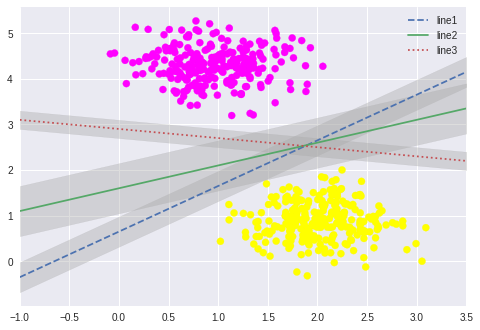
\includegraphics[width=0.8\linewidth]{svm.png}
	\caption{Svm}
	\label{fig:svm}
\end{figure}

The procedure for implementing the SVM is:

\begin{itemize}
	\item Define an optimal hyperplane: maximizing margin.
	\item Extend the above term for non-linearly separable problems; in other words have a penalty term for miss-classifications.
	\item Map data to high dimensional space where it is easier to classify with linear decision surfaces and reformulate the problem sot that the data is mapped implicitly to this space.
\end{itemize}

To implement SVM in \lstinline{rustlearn} we will need to create the model with the appropriate kernel function first and fit the model on the training data set. The SVM module in \lstinline{rustlearn} is just a wrapper over the \lstinline{libsvm} package\footnote{\href{https://www.csie.ntu.edu.tw/~cjlin/libsvm/}{libsvm}}. Observe the below snippet where the models for the different kernels are shown together.

\begin{lstlisting}[caption={chapter3\\/rustlearn\_classification\_tasks\\/src\\/trees\\.rs}]
use rustlearn::svm::libsvm::svc::{Hyperparameters as libsvm_svc, KernelType};
let svm_linear_model = libsvm_svc::new(
  4, KernelType::Linear, 3)
  .C(0.3).build();
let svm_poly_model = libsvm_svc::new(4, KernelType::Polynomial, 3)
  .C(0.3) .build();
let svm_rbf_model = libsvm_svc::new(4, KernelType::RBF, 3)
  .C(0.3).build();
let svm_sigmoid_model = libsvm_svc::new(4, KernelType::Sigmoid, 3)
  .C(0.3).build();
let svm_kernel_types = ["linear", "polynomial", "rbf", "sigmoid"];
let mut svm_model_types = [svm_linear_model, svm_poly_model, svm_rbf_model, svm_sigmoid_model];
for (kernel_type, svm_model) in svm_kernel_types.iter().zip(svm_model_types.iter_mut()) {
  svm_model.fit(&flower_x_train, &flower_y_train).unwrap();

  let prediction = svm_model.predict(&flower_x_test).unwrap();
  let acc = accuracy_score(&flower_y_test, &prediction);
  println!("Lib svm {kernel}: accuracy: {accuracy}", accuracy=acc, kernel=kernel_type);
};
\end{lstlisting}

We should be getting an output similar to below.

\begin{lstlisting}[caption={output}]
Lib svm linear: accuracy: 0.9
Lib svm polynomial: accuracy: 0.9
Lib svm rbf: accuracy: 0.8666667
Lib svm sigmoid: accuracy: 0.26666668
\end{lstlisting}


\label{sub:support_vector_machines}

\subsection{Neural Networks}%

Neural networks are a set of algorithms, modeled loosely after the human brain, that are designed to recognize patterns. One of the most popular ways of using neural networks is by grouping them in stacks. Usable networks that work are seen to be composed of several layers. The layers are made of nodes. A node is just a place where computation happens. A node combines input from the data with a set of coefficients or weights, that either amplify or dampen that input, thereby assigning significance to inputs with regard to the task the algorithm is trying to learn, for example which input is most helpful in classifying the data without error. These input weight products are summed and passed through an "activation function". Activation functions are generally non-linear and they work to determine whether and to what extent that signal should progress further through the network to affect the ultimate outcome, an example being the classification task. If the signal passes through, the neuron has been "activated". Take a look at Figure 2 to have an understanding of how a node might look like.

\begin{figure}
	\centering
	\includegraphics[width=0.8\linewidth]{single_node.png}
	\caption{single node example}
	\label{fig:single node example}
\end{figure}

A node layer is a row of those neuron like switches that turn on and off as the input is fed through the net. Each layers output is simultaneously the next layers input, starting from an initial input layer receiving the data. Pairing the models adjustable weights with input features is how we assign significance to those features with regard to how the neural network classifies and clusters input.

\begin{figure}
	\centering
	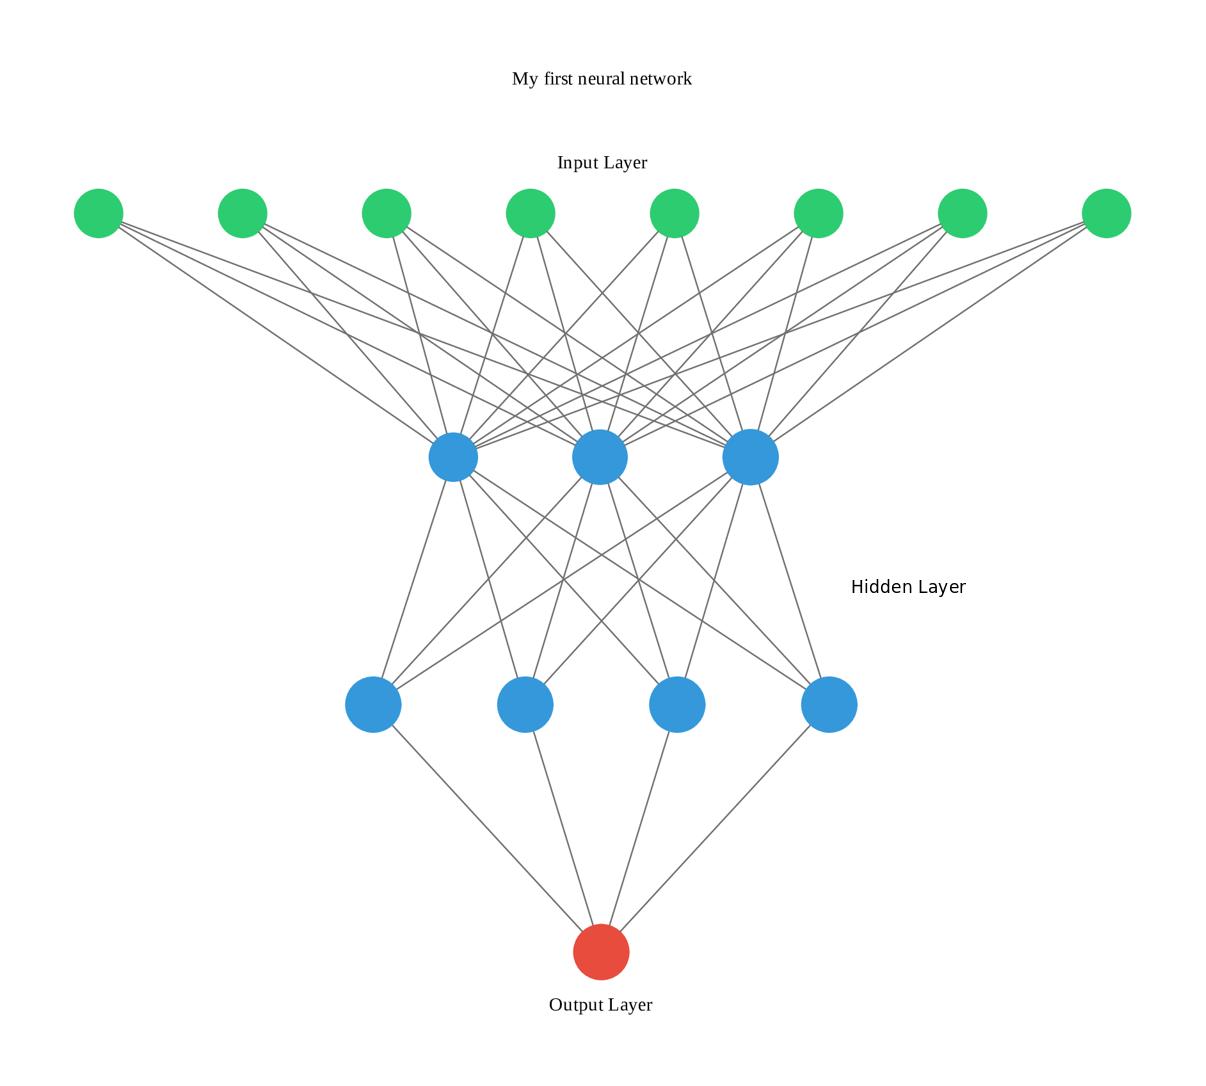
\includegraphics[width=0.8\linewidth]{deep_neural_network.png}
	\caption{deep neural network}
	\label{fig:deep neural network}
\end{figure}

Neural networks with multiple hidden layers have each layer of node train on a distinct set of features based on the previous layer's output. More deep layers learn the more complicated features in the training data, since they are able to aggregate and recombine features from the previous layers.

\paragraph{}%
\textbf{Torch and tch-rs}

Torch is a scientific computing framework with wide support for machine learning algorithms and has good support for GPU\cite{WEBSITE:12} . It is hence widely used for deep learning and creating neural network architectures. The C implementation of Torch is distributed in a package called \lstinline{libtorch}. It provides a flexible N-dimensional array or tensor, which supports basic routines for indexing. slicing, transposing, type-casting, resizing, sharing storage and cloning. This object is used by most other packages and useful and more complicated routines are built on top of it.

In Rust, the \lstinline{libtorch} C++-api has been extended using the tch-rs crate \footnote{\href{https://github.com/LaurentMazare/tch-rs}{tch-rs}}. The aim of this create is to be as close to the C++ api as possible.

To use \lstinline{tch-rs} just adding \lstinline{tch-rs} in your \lstinline{Cargo.toml} and then doing a \lstinline{cargo build} should work. In case you are in a Mac system and encounter the below error

\begin{lstlisting}[caption={}]
dyld: Library not loaded: @rpath/libmklml.dylib
  Referenced from: /path to libtorch/lib/libcaffe2.dylib
  Reason: image not found
\end{lstlisting}

We can resolve this error by manually downloading the file and adding the paths to the lib file in the mac terminal


\begin{lstlisting}[caption={installation}]
$ wget https://github.com/intel/mkl-dnn/releases/download/v0.18/mklml_mac_2019.0.3.20190220.tgz
$ gunzip -c mklml_mac_2019.0.3.20190220.tgz| tar xvf -
$ export LD_LIBRARY_PATH=/path to mkl folder/lib:"$LD_LIBRARY_PATH"
\end{lstlisting}

The code should build after this.

We will now build a small neural network on it so that the network can train on the data. To be able to do that we will need to change the data though. We will take a look at all the important steps next. These steps are under the assumption that all the data preprocessing steps are complete and are similar to the ones we encountered in the previous sections. The consolidated code is also present in the package \lstinline{iris_classification_tchrs} for reference.

First we will need to specify the test train ratio to be the same. This is a technicality that needs to be taken care because of the way matrix multiplication works and the implications we will take a look at later. So

\begin{lstlisting}[caption={iris\_classification\_tchrs}]
let test_size: f64 = 0.5;
\end{lstlisting}

Now we will need to convert the vectors to torch Tensors so that we are able to perform computations on those Tensors.

\begin{lstlisting}[caption={chapter3\\/iris\_classification\_tchrs\\/src\\/main\\.rs}]
use tch::{kind, Kind, Tensor};
let flower_x_train = Tensor::float_vec(flower_x_train.as_slice());
let flower_y_train = Tensor::float_vec(flower_y_train.as_slice()).to_kind(Kind::Int64);
let flower_x_test = Tensor::float_vec(flower_x_test.as_slice());
let flower_y_test = Tensor::float_vec(flower_y_test.as_slice()).to_kind(Kind::Int64);
\end{lstlisting}

We can now reshape the vectors to reflect the training size and the dimension of the features. Label values in this case are essentially vectors.

\begin{lstlisting}[caption={chapter3\\/iris\_classification\_tchrs\\/src\\/main\\.rs}]
let train_size = train_size as i64;
let test_size = test_size as i64;
let flower_x_train = flower_x_train.view(&[train_size, 4]);
let flower_x_test = flower_x_test.view(&[test_size, 4]);
let flower_y_train = flower_y_train.view(&[train_size]);
let flower_y_test = flower_y_test.view(&[test_size]);
\end{lstlisting}

Now we come to the actual neural network creation. Similar to figure 2 lets create a single layer network where there such that we are optimizing on the matrix equation $Y = X * W + B$ where all the values are vectors or matrices\cite{WEBSITE:14} . We will need to initiate our weights and biases for this.

\begin{lstlisting}[caption={chapter3\\/iris\_classification\_tchrs\\/src\\/main\\.rs}]
let mut ws = Tensor::ones(
  &[feature_length, 1], kind::FLOAT_CPU)
  .set_requires_grad(true);
let mut bs = Tensor::ones(
  &[train_size], kind::FLOAT_CPU)
  .set_requires_grad(true);
\end{lstlisting}

In the above example we will be setting the \lstinline{requires_grad} to be \lstinline{true} because we will need to compute the gradients for these values. Tensors have \lstinline{requires_grad} as \lstinline{false} by default and gradient for tensors for which the \lstinline{requires_grad} is false are not calculated\cite{WEBSITE:13} .

Now we will need to first perform the matrix multiplication \lstinline{flower_x_train * ws + bs}. We will then consider the loss against \lstinline{flower_y_train}. We will now need to propagate the loss. This operation will be repeated for multiple epochs and we will report the accuracy for each epoch so that we are able to keep track of increase or decrease in accuracy of the model.

\begin{lstlisting}[caption={chapter3\\/iris\_classification\_tchrs\\/src\\/main\\.rs}]
for epoch in 1..200 {
  let logits = flower_x_train.mm(&ws) + &bs;
  let loss = logits.squeeze().cross_entropy_for_logits(&flower_y_train);
  ws.zero_grad();
  bs.zero_grad();
  loss.backward();
  no_grad(|| {
    ws += ws.grad() * (-1);
    bs += bs.grad() * (-1);
  });
  let test_logits = flower_x_test.mm(&ws) + &bs;
  let test_accuracy = test_logits
    .argmax1(-1, false)
    .eq1(&flower_y_test)
    .to_kind(Kind::Float)
    .mean()
    .double_value(&[]);
  println!(
    "epoch: {:4} train loss: {:8.5} test acc: {:5.2}%",
    epoch,
    loss.double_value(&[]),
    100. * test_accuracy
  );
}
\end{lstlisting}
 
Running this model we should see incremental decrease in the loss of the model.

\label{par:}

\label{sub:neural_networks}

\subsection{Model Evaluation}%

\paragraph{Accuracy}%
The most common metric to evaluate a classification model is by using classification accuracy. It is the ratio of the number of correct predictions to the total number of input samples.

\begin{equation}
	\text{Accuracy} = \frac{\text{Number of correct predictions}}{\text{Total number of predictions made}} 
\end{equation}

We can implement this using the below function

\begin{lstlisting}[caption={ml\\-utils\\/src\\/sup\_metrics\\.rs}]
fn accuracy(y_test: &Vec<f32>, y_preds: &Vec<f32>) -> f32 {
  let mut correct_hits = 0;
  for (predicted, actual) in y_preds.iter().zip(y_test.iter()) {
    if predicted == actual {
      correct_hits += 1;
    }
  }
  let acc: f32 = correct_hits as f32 / y_test.len() as f32;
  acc
}
\end{lstlisting}

Or since we are using \lstinline{rustlearn} in this chapter we can use the \lstinline{accuracy_score} from the package.

\begin{lstlisting}[caption={chapter3\\/rustlearn\_classification\_tasks\\/src\\/logistic\_reg\\.rs}]
use rustlearn::metrics::accuracy_score;

let prediction = model.predict(&flower_x_test).unwrap();
let acc = accuracy_score(&flower_y_test, &prediction);
\end{lstlisting}

Using the above function we should be able to see the following accuracy scores for the models implemented.

\begin{lstlisting}[caption={chapter3\\/rustlearn\_classification\_tasks\\/src\\/logistic\_reg\\.rs}]
$ cargo run lr < data/iris.csv
    Finished dev [unoptimized + debuginfo] target(s) in 3.66s
     Running `target/debug/rustlearn_classification_tasks lr`
Logistic Regression: accuracy: 0.3
Logistic Regression: accuracy: 0.3
\end{lstlisting}

This method of calculating the accuracy score only works if there are equal number of samples belonging to each class. For example lets assume that $99\%$ samples belong to class A and the remaining $1\%$ belong to class B. Then by the above metric a simple model, such as below, that predicts all out of sample classes as class A would have an accuracy of $99\%$.

\begin{lstlisting}[caption={my awesome machine learning model}]
fn model(y_test: &Vec<f32>) -> Vec<String> {
  vec![String::from("Class A"); y_test.len()]
}
\end{lstlisting}

The result would be that we would have a false sense of achieving high accuracy.
\label{par:accuracy}

\paragraph{Logarithmic Loss}%
Logarithmic loss or cross entropy loss, works by penalizing the false classifications. It works well for multi-class classifications. Log Loss increases as the predicted probability diverges from the actual label. An perfect model would have a log loss of 0. So predicting a probability of 0.12 when the actual observation label is 1 would be bad and result in high log loss\cite{WEBSITE:15} . This is given by

\begin{equation}
	H_p(q) = - \frac{1}{N}\sum_{i=1}^{N}y_i \cdot \log(p(y_i)) + (1-y_i) \dot \log(1-p(y_i))
\end{equation}

The graph below shows the range of possible log loss given a true observation of $1$. Log loss is not very steep when the probability is approaching 1 but increases rapidly when the probability is going towards 0. We want the behaviour to be penalized for any errors, but notice how the penalizing is infinite when the predictors are confident and wrong.

\begin{figure}[htpb]
	\centering
	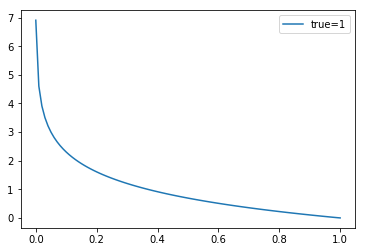
\includegraphics[width=0.8\linewidth]{logloss.png}
	\caption{logloss}
	\label{fig:logloss}
\end{figure}

Thus log loss has a more nuanced approach to accuracy than a simple yes no nature. It gives a value based on how wrong the model is from the true value.

In Rust the below function will calculate the log-loss score. The vectors \lstinline{y_test} and \lstinline{y_preds} are the ground truths and the predicted values. Log-loss is undefined for probability values of 0 and 1 and hence the \lstinline{y_test} vector is clamped to a little above 0 and a little below 1 given by \lstinline{eps} following the equation $\max(\min(p, 1 - \epsilon), \epsilon)$. Note that \lstinline{partial_cmp} is used to compare as we are comparing between two floats. Rust official stance is that comparing floating point numbers is very tricky and situation dependent, and best avoided if at all possible. There is no panacea that "just works"\cite{WEBSITE:16} .

Once done we will implement the actual log-loss function for binary classification on the clamped vector.

\begin{lstlisting}[caption={ml\\-utils\\/src\\/sup\_metrics\\.rs}]
fn logloss_score(y_test: &Vec<f32>,
                 y_preds: &Vec<f32>,
		 eps: f32) -> f32 {
  let y_preds = y_preds.iter().map(|&p| {
    match p.partial_cmp(&(1.0 - eps)) {
      Some(Ordering::Less) => p,
      _ => 1.0 - eps, // if equal or greater.
    }
  });
  let y_preds = y_preds.map(|p| {
    match p.partial_cmp(&eps) {
        Some(Ordering::Less) => eps,
        _ => p,
    }
  });

  let logloss_vals = y_preds.zip(y_test.iter())
    .map(|(predicted, &actual)| {
      if actual as f32 == 1.0 {
        (-1.0) * predicted.ln()
      } else if actual as f32 == 0.0 {
        (-1.0) * (1.0 - predicted).ln()
      } else {
        panic!("Not supported. y_preds should be either 0 or 1");
      }
    });
  logloss_vals.sum()
}
\end{lstlisting}

This can now be used in something similar to below.

\begin{lstlisting}[caption={}]
let preds = vec![1., 0.0001, 0.908047338626,
  0.0199900075962, 0.904058545833, 0.321508119045,
  0.657086320195];
let actuals = vec![1., 0., 0., 1., 1., 0., 0.];
println!("{:?}",
  logloss_score(&actuals, &preds, 1e-15)); // output 7.8581247
\end{lstlisting}
\label{par:logarithmic_loss}

% TODO: implement confusion matrix
%\paragraph{Confusion Matrix}%
%Confusion matrix is a table with rows and columns that report the number of false positives, false negatives, true positives, and true negatives. This allows for a more detailed analysis than the mere proportions of correct classifications. An example of a confusion matrix is sown below.
%
%\begin{center}
%\begin{tabular}{ |c|c|c|c| }
%\hline
%actual/predicted & negative & positive \\
%\hline
%Negative & a & b \\
%Positive & c & d \\
%\hline
%\end{tabular}
%\end{center}
%
%Confusion matrix is implemented in 
%
%\label{par:confusion_matrix_}

\paragraph{ROC-AUC}%
An ROC curve(receiver operating characteristic curve) is a graph showing the performance of a classification model at all classification thresholds\cite{WEBSITE:17}. The curve plots two parameters.

\begin{itemize}
	\item True Positive Rate
	\item False Positive Rate
\end{itemize}

True Positive Rate(TPR) is a synonymn for recall and is therefore defined as

\begin{equation}
	\text{TPR} = \frac{\text{TP}}{\text{TP + FN}} 
\end{equation}

and False Positive Rate is defined as

\begin{equation}
	\text{FPR} = \frac{FP}{\text{FP + TN}}
\end{equation}

An ROC curve  plots TPR vs FPR at different classification thresholds. Lowering the classification threshold classifies more items as positive, thus increasing both false positives and true positives.

\begin{figure}[htpb]
	\centering
	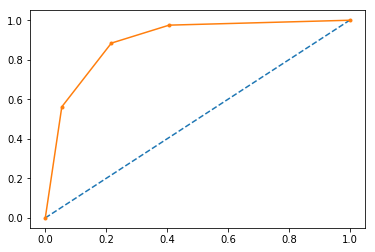
\includegraphics[width=0.8\linewidth]{rocauc.png}
	\caption{roc-auc curve} 
	\label{fig:rocauc}
\end{figure}

AUC stands for "Area under the ROC Curve". It measures the entire two dimensional area under the entire ROC Curve. For the figure 5 the ROC-AUC area is 0.895. As evident the score has a range between 0 and 1. The greater the value, the better is the performance of the model.

The crate \lstinline{rustlearn} has roc-auc score implemented for binary classification.

\begin{lstlisting}[caption={chaper3\\/rustlearn\_classification\_tasks\\/src\\/binary\_class\_scores\\.rs}]
use rustlearn::metrics::roc_auc_score;
let preds = vec![1., 0.0001, 0.908047338626, 0.0199900075962,
  0.904058545833, 0.321508119045, 0.657086320195];
let actuals = vec![1., 0., 0., 1., 1., 0., 0.];
println!("roc auc scores: {:?}",
  roc_auc_score(&Array::from(actuals), &Array::from(preds))?); // output: 0.6666667 
\end{lstlisting}

Running the above should give something like below.

\begin{lstlisting}[caption={chaper3\\/rustlearn\_classification\_tasks\\/src\\/binary\_class\_scores\\.rs}]
$ cargo run bs
    Finished dev [unoptimized + debuginfo] target(s) in 0.16s
     Running `target/debug/rustlearn_classification_tasks bs`
logloss score: 7.8581247
roc auc scores: 0.6666667
\end{lstlisting}
\label{par:roc_auc}

%% % https://towardsdatascience.com/metrics-to-evaluate-your-machine-learning-algorithm-f10ba6e38234
%% % https://machinelearningmastery.com/how-to-score-probability-predictions-in-python/
%% % https://medium.com/datadriveninvestor/how-to-evaluate-the-performance-of-a-machine-learning-model-45063a7a38a7
%% % https://towardsdatascience.com/metrics-to-evaluate-your-machine-learning-algorithm-f10ba6e38234
%% % https://www.analyticsvidhya.com/blog/2016/02/7-important-model-evaluation-error-metrics/
%
%
%
%\label{sub:model_evaluation}

\label{sec:classification}

\section{Conclusion}%
This chapter introduced you to different classification models that can be implemented in Rust such as logistic regression, decision trees, random forest, xgboost and neural networks. We look at the code for creating these models using different Rust packages, \lstinline{rustlearn}, \lstinline{rust-xgboost} and \lstinline{tch-rs}. Finally we looked at different accuracy measures for evaluating the quality of these classification models in Rust.

In the next chapter you will learn about creating unsupervised models in Rust.

\label{sec:conclusion}

\printbibliography
\nocite{*}

\end{document}
